% !TEX program = xelatex
\documentclass[UTF8]{ctexart}
\usepackage{amsmath}
\usepackage{graphicx}

\usepackage{geometry}
\geometry{top=20mm,bottom=20mm,left=20mm,right=20mm}

\usepackage{fancyhdr}
\pagestyle{fancy}
\fancyhead{}
\fancyhead[C]{\bf \footnotesize SYSU Collegiate Programming Contest 2020, Online}
\fancyfoot[C]{\bf \thepage}
\setlength{\topmargin}{-20mm}

\title{\bf SYSU Collegiate Programming Contest 2020, Online}
\author{}
\date{\bf November 14, 2020}

\renewcommand\contentsname{}
\renewcommand\thesection{\Large \Alph{section}.}

\def\problem#1{\clearpage \section{\Large \bf #1}}
\def\subitem#1{\noindent{\large \bf \\#1}\nopagebreak}
\def\input{\subitem{Input}}
\def\output{\subitem{Output}}
\def\sample{\subitem{Sample}}
\def\note{\subitem{Note}}
\def\source{\subitem{Source}}
\def\tabincell#1#2{\begin{tabular}[t]{@{}#1@{}}#2\end{tabular}}

\begin{document}
\maketitle
\tableofcontents
\thispagestyle{fancy}

%-----

\problem{Welcome to SYSU}

Sun Yat-sen University, originally known as National Guangdong University, was founded in 1924 by Dr. Sun Yat-sen (also called Sun Zhongshan), a great democratic revolutionary leader of the 20th century. The University is located in Guangdong Province, an area neighboring Hong Kong and Macao, which is at the forefront of China's reform and opening up.

\begin{center}
	
\includegraphics[width=0.618\textwidth]{welcome.jpg}
\end{center}

Being one of the leading universities in the People's Republic of China, Sun Yat-sen University is a comprehensive multi-disciplinary university, including the humanities, social sciences, natural sciences, technical sciences, medical sciences, pharmacology, and management science. At present, Sun Yat-sen University covers a total area of 6.17 square kilometers and has 4 campuses: Guangzhou South Campus, Guangzhou North Campus, Guangzhou East Campus, and Zhuhai Campus.

\input

The input contains a positive integers n.

$1\le n\le 12$

\output

You should output the lexicographically N-th string with the same letters (2*`S'+1*`Y'+1*`U') as ``SYSU''.

\sample

\noindent\begin{tabular}{|p{5cm}|p{5cm}|} \hline
	Input            & Output              \\ \hline
	\tabincell{l}{1} & \tabincell{l}{SSUY} \\ \hline
	\tabincell{l}{5} & \tabincell{l}{SYSU} \\ \hline
\end{tabular}

\source

吴坎

%-----

\problem{Formula}

This formula is written as an equation about the length of edges A, B and C, which is usually called Pythagorean law.

$A^2 + B^2 = C^2$

Where $C$ is the length of the slanted side and $A$ and $B$ are the lengths of the other two sides.

Given $n$, you need to compute right triangles with side lengths $A$, $B$ and $C$ satisfying inequality $1 \le A \le B \le C \le n$.

\input

The first line of input contains an integer $n~(1\leq n\leq 10000)$.


\output

The first line of input contains an integer donating the answer.

\sample

\noindent\begin{tabular}{|p{5cm}|p{5cm}|} \hline
	Input            & Output           \\ \hline
	\tabincell{l}{5} & \tabincell{l}{1} \\ \hline
\end{tabular}

\note

3, 4, 5

\source

范俭豪

%-----

\problem{Island}

A tour group is trapped on an island. The island can be regarded as a matrix of equal side length.

Each grid is either an obstacle (character `\#'), a tourist (character `O'), or an open space (character `.'), visitors can walk up, down, left, right(to neighboring grid), but can't walk over obstacles.

Ask how many tourists can never get out of the island.

\input

First line of the input is an integer $T$($1\le T \le 10$) indicating the number of test cases.

For each case, the first line contains an integer $n$ ($1\le n \le 50$) indicating the side length of island, each of the following $n$ lines contains a string with exact n charactors(obstacle `\#', tourist `O' or space `.').


\output

For each case output one integer, the number of tourist(s) cannot get out of the island.

\sample

\noindent\begin{tabular}{|p{5cm}|p{5cm}|} \hline
	Input & Output         \\ \hline
	\tabincell{l}{
		1                      \\
		4                      \\
		O.\#\#                 \\
		.\#O\#                 \\
		\#O.\#                 \\
		.\#\#\#
	}     & \tabincell{l}{
		2
	}                      \\ \hline
\end{tabular}

\source

梁赛波

%-----


\problem{Liz and the Blue Bird}

After a long thought, Liz made a tough decision. When the girl came back home from picking raspberries with delight. Liz said goodbye to the girl with smile. A basket of raspberries dropped, scattering on the floor. ``You are ought to be free and use your lightsome wings to fly to everywhere you want.'' ``Why? I just want to stay with you forever. Only by your side can I taste the sweet of happiness.'' ``I am the cage that traps you. You have wings and vast sky to explore. I can't deprive you of your wings,'' Liz opened the door, smiling mildly. ``So just leave here and fly high. Please let me watch your beautiful figure go away,'' Liz held out her hand, ``That's the way I convey my feelings.'' She paused and took a deep breath ``I love you.'' The girl sobbed, stepped slowly towards door. She looked back, with love, with unwillingness, and turned into a blue bird, flying away.

\begin{center}
	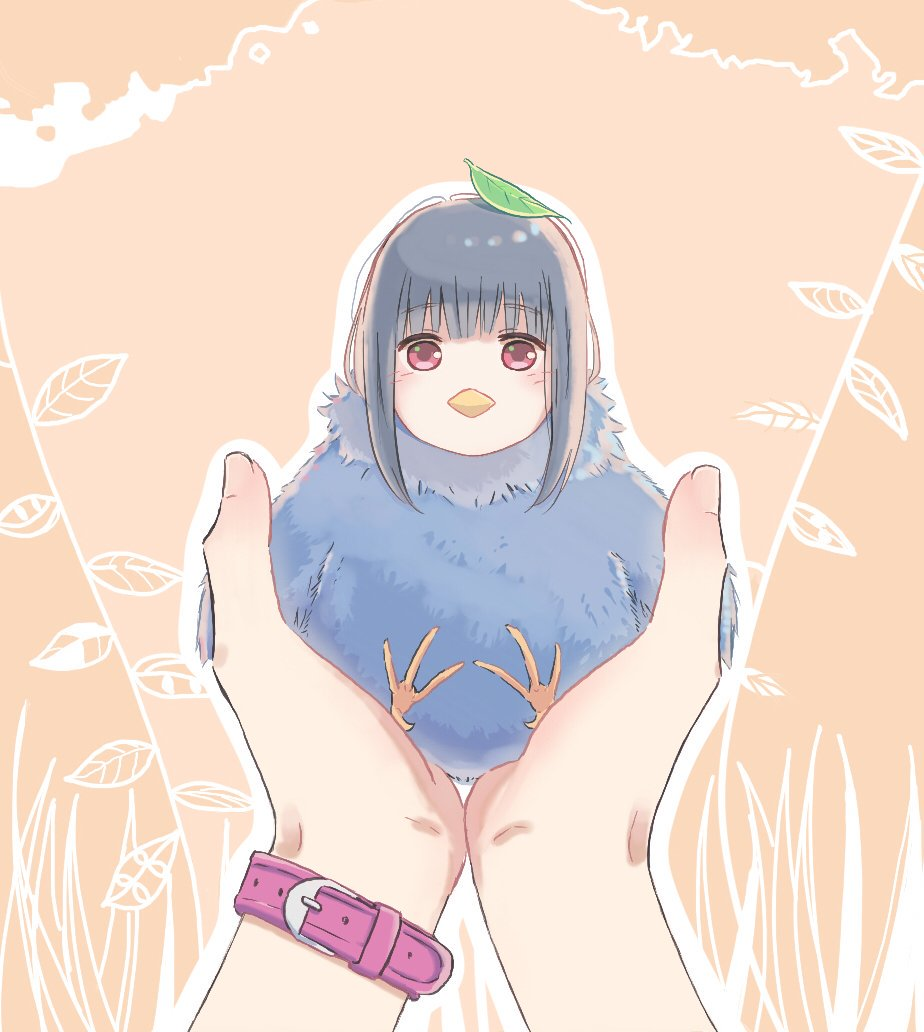
\includegraphics[width=0.618\textwidth]{bluebird.jpg}
\end{center}

After the blue bird flew away, Liz still missed her very much. Worrying that she and other small animals might be caught in a storm again, Liz decided to transplant trees in the woods to cover as much area as possible. There were $n$ trees in the woods, and each tree $T_i$ can be represented as a closed interval $[a_i,b_i]$. Liz wanted to find a solution so that all intervals covered $[0,10000]$, and the displacement of the interval with the largest displacement was minimized. Specifically, suppose $T_i$ was moved to $[a_i+c_i, b_i+c_i]$, and Liz wanted to minimize $\max_i\lvert c_i \rvert$.


\input

First line of the input is an integer $n$ indicating the number of trees.

The following $n$ lines, each line contains 2 integers $a_i,b_i$.

$1<n<10000, 0\le a_i<b_i\le 10000, \sum_{i=1}^n(b_i-a_i)\ge 10000$

\output

Output a real number that represents the answer.

If the answer is an integer, output the integer directly; otherwise, keep 1 decimal place.

If you still have any questions, you can refer to the sample output.

\sample

\noindent\begin{tabular}{|p{5cm}|p{5cm}|} \hline
	Input & Output         \\ \hline
	\tabincell{l}{
		2                      \\
		10 5010                \\
		4980 9980
	}     & \tabincell{l}{
		20
	}                      \\ \hline
	\tabincell{l}{
		4                      \\
		0 4000                 \\
		3000 5000              \\
		5001 8000              \\
		7000 10000
	}     & \tabincell{l}{
		0.5
	}                      \\ \hline
\end{tabular}

\note

The answer must be a semi-integer, that is, twice the number must be an integer.

\source

吴坎

%-----


\problem{Berth Allocation}

In a container terminal, the bottleneck of the traffic is often at the quay. Therefore, the terminal operator has to allocate a limited number of berths of the quay to vessels in an efficient way.

\begin{center}
	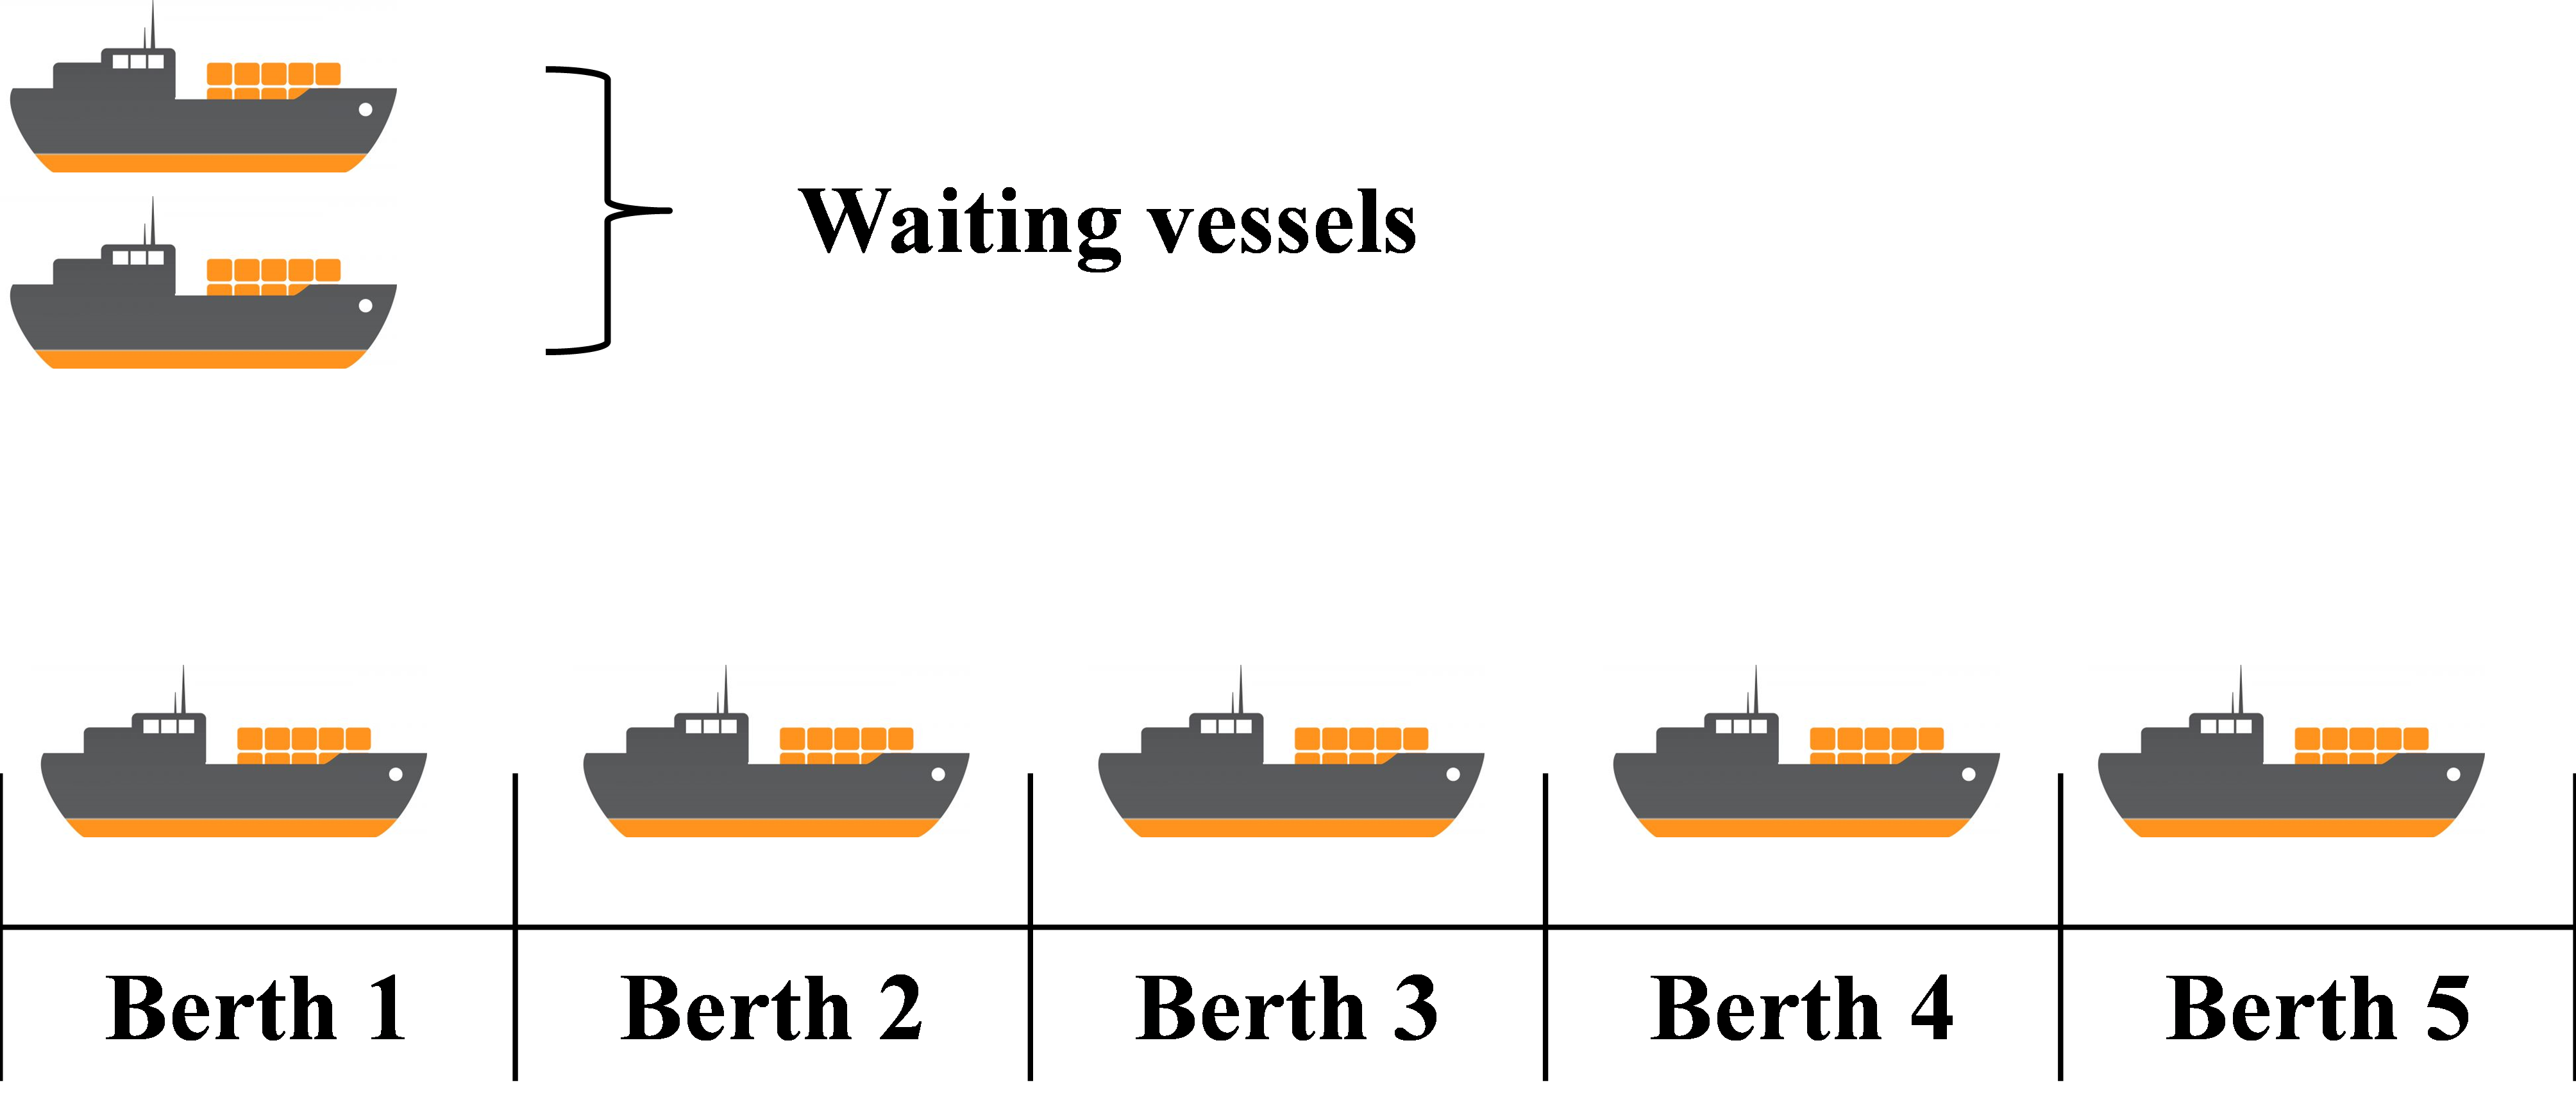
\includegraphics[width=0.618\textwidth]{berth.png}
\end{center}

As illustrate in Figure above (An illustrated example, with a quay of $n=5$ berths, $m=7$ vessels, where two vessels are waiting outside the quay), consider a container terminal of $n$ berths and $m$ vessels arrived, where each vessel $i$ (for $i=1,2,\ldots,m$) requires a berth to load and unload containers, and the handling time is $t_{i,j}$ minutes if berth $j$ (for $j=1, 2, \ldots, n$) is allocated to vessel $i$. For each vessel $i=1,2,\ldots,m$, the terminal manager, Brother D, needs to decide on the berth, denoted by $b_i\in\{1,2,\ldots,n\}$, as well on the starting time of berthing, denoted by $s_i\ge 0$. It must be satisfied that no two vessels are allowed to occupy the same berth simultaneously, i.e., for any two different vessels i and j, if $b_i=b_j$, then either $s_i+t_{i,b_i}\le s_j$ or $s_j+t_{j,b_j}\le s_i$ must be satisfied. Your task is to help Brother D to minimize the total completion time of the vessels, i.e., to minimize $\sum_{i=1}^m(s_i+t_{i,b_i})$.

\input

First line of the input is an integer $T$ indicating the number of test cases. For each case, the first line contains two integers $n$ and $m$ (for $1\le n\le 50, 1\le m\le 200$). Each of the following $m$ lines contains $n$ positive integers representing vessel i's handling times $t_{i1}, t_{i2}, \ldots, t_{i,m} (t_{i,j} \le 1000)$.

\output

For each case, output one integer, the minimum total weighted completion time of all the vessels.

\sample

\noindent\begin{tabular}{|p{5cm}|p{5cm}|} \hline
	Input & Output         \\ \hline
	\tabincell{l}{
		1                      \\
		5 7                    \\
		1 2 3 4 5              \\
		2 1 3 4 5              \\
		2 3 1 4 5              \\
		2 3 4 1 5              \\
		2 3 4 5 1              \\
		2 2 2 2 2              \\
		2 2 2 2 2
	}     & \tabincell{l}{
		11
	}                      \\ \hline
\end{tabular}

\source

吴坎

\end{document}
